
\documentclass[12pt]{article}

\usepackage[utf8]{inputenc}
\usepackage[bulgarian]{babel}
\usepackage{graphicx}
\usepackage{sidecap}  %required for side captions
\usepackage{amssymb}
\usepackage{amsmath}
\usepackage{hyperref}
\usepackage{commath}  
\usepackage[top=1.3in, bottom=1.5in, left=1.3in, right=1.3in]{geometry}


\begin{document}
	\begin{center}
        \LARGE{\textbf{Тема: Разширение на проект от УЕБ: PIC2MAP - сайт за позициониране на снимки по GPS координати}
        
        \bigskip
        \Large{Предмет: AWS}
        
        \medskip
        \Large{Изготвил: Виолета Павлова, фн: 81872, имейл: violetaip@uni-sofia.bg}
        
        \medskip
        \Large{Лектор: доц. д-р Милен Петров, година: 2022}
        
        \bigskip
	\end{center}
    
    
  %  \newpage
    \tableofcontents
    \bigskip
    \bigskip
    \newpage
  
\section{Условие} 

\noindent Настоящето задание е създаването на приложение, подобно на \newline
https://www.pic2map.com/tnbzb.html, което съдържа следната функционалност:
\begin{itemize}
    \item Регистрация в приложението
    
    \item Вход в приложението
    
    \item Възможност за преглед върху публична карта (напр. openstreet map). Картата се поставя на заден фон, когато потребителят кликне върху някоя отметка и се визуализира съответстващата й картинка.
    
    \item Снимките могат да бъдат качвани като частни или публични, с възможност да се преглеждат на карта;
    
    \item Качване на снимка чрез специална за целта форма или чрез кликване върху картата. Снимката може да се 'оразмерява' по зададен формат (insta formats). Ако качената снимка съдържа информация за местоположението на заснемане, то тези координати се взимат предвид. 
\end{itemize}

\medskip

\section{Въведение}

Целта на проекта е да се разработи уеб приложение за споделяне на снимки. След поредното си пътуване, човек ще може да качи любими снимки от местата, на които е бил. Много от тези снимки вече имат GPS координати, но в случай, че нямат, човек може да избере къде да постави своята снимка на картата . Ще може да избере дали иска неговата снимка да е публична, като така допринася към всеобщата колекция от снимки. Ако реши, че снимката е много лична, потребителят може да запази само за себе си, като я направи частна. Приложението дава възможност за виртуална разходка из забележителностите на всяка точка от земята. Приложението може да се ползва и от нерегистрирани потребители, като те могат само да разглеждат публичните снимки.
\newpage
\section{Теория}
За разширяването на приложението се използват три AWS услуги:
\medskip\newline
\noindent \textbf{Amazon Elastic Compute Cloud (EC2):} уеб услуга, която осигурява сигурен и преоразмерим изчислителен капацитет в облака чрез използване на виртуални машини. Предоставя лесна интеграция с други AWS услуги, например AWS RDS чрез VPC (частна виртуална мрежа в облака на Amazon). Настоящото приложение върви на EC2 инстанция, като има връзка с друга RDS инстанция.
\medskip\newline
\noindent \textbf{Amazon Relational Database Service (RDS):} услуга, която позволява лесно създаване, конфигуриране и мащабиране на релационни бази данни. RDS се грижи за голяма част от административните задачи по поддържането на базата като например създаването на backup, snapshots, security updates и т.н. Приложението съхранява изнформация за потребителите и параметрите на изображенията в RDS инстанция, която има една база данни pin-your-pics и съответно две таблици pics и users.
\medskip\newline
\noindent \textbf{AWS Simple Storage Service (S3):} услуга, която предоставя сигурно и надеждно съхраняване на обекти в облака. Това е интерфейс, който позволява съхраняването и достъпването на голямо количество ресурси. Могат да се съхраняват най-обикновени текстови файлове или по-специални файлове, снимки, видеоматериали. В контекста на приложението е удобно съхраняването на изображенията, които са разпръснати из картата. Тези изображения се достъпват и качват в S3 bucket-a бързо и лесно.
\medskip

\medskip

%\newpage

\section{Използвани технологии}
\textbf {Development}:
\begin{itemize}
\item \textbf{Frond-end}: HTML5, CSS3, JavaScript
\item \textbf{Back-end}: PHP version 'PHP 8.0.18'
\item \textbf{Database}: MySQL
\end{itemize}
\textbf{AWS}:
\begin{itemize}
\item  RDS
\item  EC2
\item  S3
\end{itemize}

\newpage

\section{Инсталация и настройки}
\subsection{IAM}
Разбира се всички стъпки изпълняваме с IAM user, на който root user-a закача съответните policies, които да го упълномощават да извършва операциите по инстанциите. Правата са следните: AmazonRDSFullAccess, AmazonEC2FullAccess, AmazonS3FullAccess.
\subsection{RDS}
  В AWS console създаваме RDS инстанция с free tier, като указваме master username и password, които ще използваме за връзка с базата. Освен това по време на създаването на инстанцията създаваме security group pin-your-pics-security-group, която в последствие ще дадем и на EC2 инстанцията. След като сме създали инстанцията, в кода connect.inc.php обновяваме данните за достъп до базата, която вече е нашата RDS инстанция. 

\begin{figure}[!htb]
    \centering
        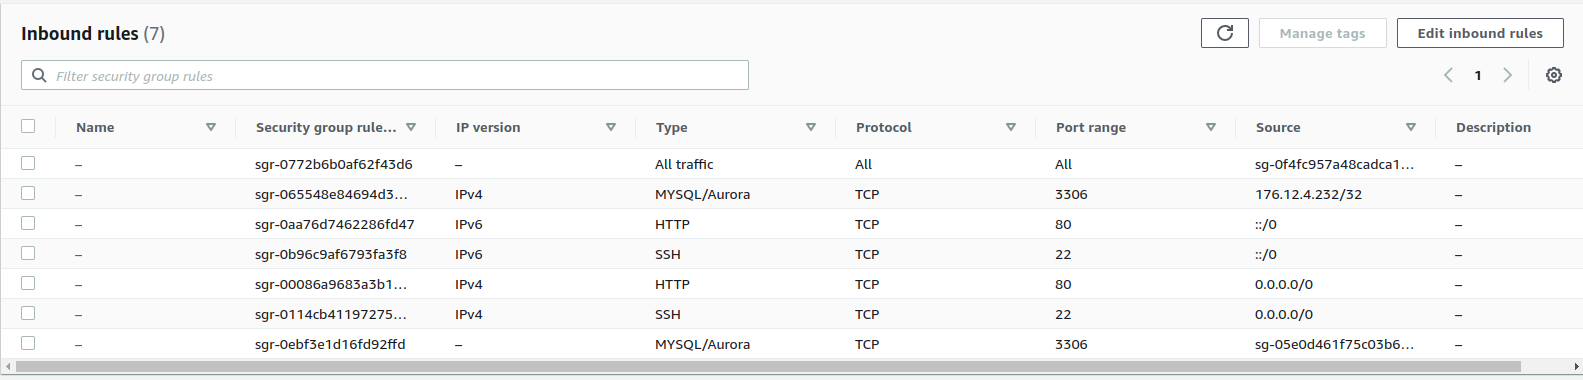
\includegraphics[scale=0.30]{inbound-rules.png}
        \caption{Настройки на \textbf{pin-your-pics-security-group}, достъпни през VPC Security groups}
\end{figure}

\subsection{EC2}
 В AWS console създаваме EC2 инстанция c free tier в pin-your-pics-security-group. Инстанцията се намира в същия VPC като RDS. \\
 Свързваме се с виртуалната машина чрез EC2InstanceConnect или SSH. \\
 Инсталираме php, mysql, apache: \\
 > sudo yum install php8.0 \\
 > sudo yum install mysql \\
 > sudo apt install apache2 \\
 Стартираме сървъра: \\
 > sudo systemctl start httpd \\
 Свързваме се с RDS инстанцията чрез следната команда: \\
 > mysql -h <endpoint> -P <port> -u <username> -p \\
 endpoint и port взимаме от RDS, default port e 3306. Username e master username, a за password въвеждаме master password.
 След успешно свързване с базата изпълняваме скрипта (dbcreate.sql) за създаване на database и двете таблици в нея. \\
 Клонираме github repository-то: \\
 > git clone https://github.com/samoleti/pin-your-pics.git \\
 Копираме проекта: \\
 > sudo cp -r pin-your-pics /var/www/html \\
 Настройваме пътя за приложението за Apache във файла /etc/httpd/conf/httpd.conf, като обновяваме DocumentRoot /var/www/html/pin-your-pics/htdocs. \\
 Необходимо ни е да инсталираме composer: \\
 > php -r "copy('https://getcomposer.org/installer', 'composer-setup.php');" \\
 > php -r "if (hash\_file('sha384', 'composer-setup.php') === \\ '55ce33d7678c5a611085589f1f3ddf8b3c52d662cd01d4ba75c0ee0459970c2200a51f492d557530c71c15d8dba01eae') { echo 'Installer verified'; } else { echo 'Installer corrupt'; unlink('composer-setup.php'); } echo PHP\_EOL;"
  php composer-setup.php \\
 > php -r "unlink('composer-setup.php');" \\
 Инсталираме Amazon SDK for PHP: \\ 
 > composer require aws/aws-sdk-php \\
Приложението можем да достъпим чрез Public IPv4 DNS. Например настоящето приложение е достъпно на адрес: \\
 http://ec2-3-223-135-185.compute-1.amazonaws.com/
 
 
\subsection{S3}
Създаваме S3 bucket инстанция, която в последствие се ползва от приложението чрез s3 client. \\
В кода във файловете upload.inc.php, index.php за bucket, IAM\_KEY, IAM\_SECRET на местата на звездичките пишем името на новосъздадения bucket и credentials на IAM user-a, чрез който сме създали bucket-a.\\
Другият вариант е да даваме достъп на EC2 инстанцията до S3 bucket: \\
https://aws.amazon.com/premiumsupport/knowledge-center/ec2-instance-access-s3-bucket/ \\
По този начин избягваме писането на credentials.

\newpage


\medskip

\section{Кратко ръководство за потребителя}
\begin{figure}[!htb] 
    \centering
        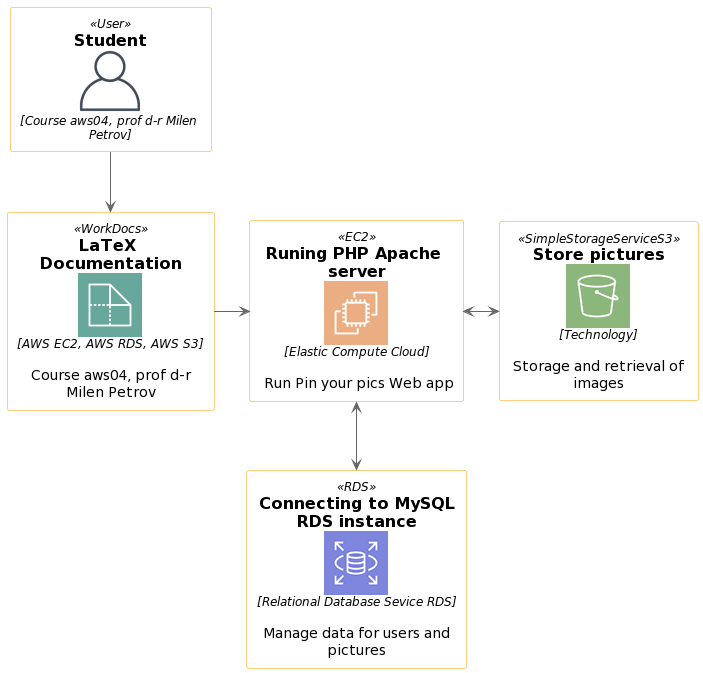
\includegraphics[scale=0.55]{diagram-docs.png}
        \newline \caption{UML диаграма}
\end{figure}
\section{Примерни данни}

Потребител: \\
username: samoleti \\
email: leti1999@abv.bg	\\
password: 1234 \\
За снимки с GPS локация в EXIF метаданните си използвах примерните изображения от https://github.com/samoleti/pin-your-pics/tree/master/samples

 
\section{Описание на програмния код}

Сървърната част се намира в папката pin-your-pics/php. Помощните php файлове, които не са отделни страници се намират в pin-your-pics/php/includes папката.
\newline
Базата от данни се състои от две таблици - users и pics. Таблицата users съдържа информацията за регистрираните потребители. Таблицата users съдържа информация за GPS локацията на снимката, кой е авторът, къде на сървъра се пази снимката и дали е частна/публична.
\newline
JavaScript кодът се намира в папката pin-your-pics/js папката, която се изпълнява на клиента. Той отговаря за извършването на заявки към сървърната част.
\newline
CSS файловете са в в папката pin-your-pics/css, с които допълнително се стилизира уеб страницата. 


\medskip


\section{Приноси на студента, ограничения и възможности за бъдещо развитие}

Представената функционалност е разработена от автора на документа. \\
Възможност за бъдещо подобрение е добавянето на затворени групи за споделяне на снимки. Друга възможност е използването на снимка/карта вместо конкретно географска такава. Откъм услуги в облака е добра стъпка използването на AWS CodeCommit.

\medskip

\section{Какво научих}
Разширяването на проекта чрез AWS услуги ме научи как да създам уеб приложение, качено в облака. За мен беше интересно да науча как да комбинирам набор от AWS услуги и как те си взаимодействат помежду си.

\section{Списък с фигури и таблици}

\listoffigures

\section{Използвани източници}

\noindent\href{https://learn.fmi.uni-sofia.bg/course/view.php?id=8205}{[1] FMI Moodle course}
\newline
\noindent\href{https://awsacademy.instructure.com/courses/15596}{[2] AWS Academy Introduction to Cloud: Semester 1}
\newline
\noindent\href{https://awsacademy.instructure.com/courses/15407}{[3] AWS Academy Introduction to Cloud: Semester 2}

\noindent\href{https://aws.amazon.com/premiumsupport/knowledge-center/ec2-instance-access-s3-bucket/}{[4] Grant EC2 instance access to S3 bucket/}
 
\medskip



\bigskip


\end{document}